% Options for packages loaded elsewhere
\PassOptionsToPackage{unicode}{hyperref}
\PassOptionsToPackage{hyphens}{url}
%
\documentclass[
]{article}
\usepackage{lmodern}
\usepackage{amssymb,amsmath}
\usepackage{ifxetex,ifluatex}
\ifnum 0\ifxetex 1\fi\ifluatex 1\fi=0 % if pdftex
  \usepackage[T1]{fontenc}
  \usepackage[utf8]{inputenc}
  \usepackage{textcomp} % provide euro and other symbols
\else % if luatex or xetex
  \usepackage{unicode-math}
  \defaultfontfeatures{Scale=MatchLowercase}
  \defaultfontfeatures[\rmfamily]{Ligatures=TeX,Scale=1}
\fi
% Use upquote if available, for straight quotes in verbatim environments
\IfFileExists{upquote.sty}{\usepackage{upquote}}{}
\IfFileExists{microtype.sty}{% use microtype if available
  \usepackage[]{microtype}
  \UseMicrotypeSet[protrusion]{basicmath} % disable protrusion for tt fonts
}{}
\makeatletter
\@ifundefined{KOMAClassName}{% if non-KOMA class
  \IfFileExists{parskip.sty}{%
    \usepackage{parskip}
  }{% else
    \setlength{\parindent}{0pt}
    \setlength{\parskip}{6pt plus 2pt minus 1pt}}
}{% if KOMA class
  \KOMAoptions{parskip=half}}
\makeatother
\usepackage{xcolor}
\IfFileExists{xurl.sty}{\usepackage{xurl}}{} % add URL line breaks if available
\IfFileExists{bookmark.sty}{\usepackage{bookmark}}{\usepackage{hyperref}}
\hypersetup{
  pdftitle={Trabajo práctico N°3: Machine Learning},
  pdfauthor={Gino Avanzini; Emiliano Cabrino; Adrián Cantaloube; Gonzalo Fernández},
  hidelinks,
  pdfcreator={LaTeX via pandoc}}
\urlstyle{same} % disable monospaced font for URLs
\usepackage{graphicx,grffile}
\makeatletter
\def\maxwidth{\ifdim\Gin@nat@width>\linewidth\linewidth\else\Gin@nat@width\fi}
\def\maxheight{\ifdim\Gin@nat@height>\textheight\textheight\else\Gin@nat@height\fi}
\makeatother
% Scale images if necessary, so that they will not overflow the page
% margins by default, and it is still possible to overwrite the defaults
% using explicit options in \includegraphics[width, height, ...]{}
\setkeys{Gin}{width=\maxwidth,height=\maxheight,keepaspectratio}
% Set default figure placement to htbp
\makeatletter
\def\fps@figure{htbp}
\makeatother
\setlength{\emergencystretch}{3em} % prevent overfull lines
\providecommand{\tightlist}{%
  \setlength{\itemsep}{0pt}\setlength{\parskip}{0pt}}
\setcounter{secnumdepth}{-\maxdimen} % remove section numbering

\title{Trabajo práctico N°3: Machine Learning}
\author{Gino Avanzini \and Emiliano Cabrino \and Adrián Cantaloube \and Gonzalo Fernández}
\date{}

\begin{document}
\maketitle

\hypertarget{implementaciuxf3n-de-una-red-neuronal-tipo-multi-layer-perceptron-mlp}{%
\section{Implementación de una red neuronal tipo multi-layer perceptron
(MLP)}\label{implementaciuxf3n-de-una-red-neuronal-tipo-multi-layer-perceptron-mlp}}

El objetivo de este ejercicio es implementar un MLP y entrenar la red
con distintos problemas. En primera instancia se intentará predecir el
valor de casas con el famoso
\href{../TP_3/datasets/USA_Housing.csv}{dataset de ``USA Housing''}.
Luego se entrenará la red con un
\href{../TP_3/datasets/pendulum.csv}{dataset} generado a partir del
controlador difuso para el péndulo invertido realizado en el trabajo
práctico 2. De esta forma se intentará controlar el péndulo con la red
neuronal.

\hypertarget{topologuxeda-de-la-red}{%
\subsection{Topología de la red}\label{topologuxeda-de-la-red}}

El MLP implementado es una red neuronal con 3 capas: una de entrada, una
de salida y una capa oculta. La cantidad de neuronas en la capa oculta
se deja como parámetro mientras que la cantidad de neuronas de entrada y
de salida son variables de acuerdo al problema. En el caso de USA
Housing hay 5 entradas y una salida mientras que para el control del
péndulo invertido hay dos entradas y una salida.

En cuanto a las funciones de activación, para la capa oculta se utilizó
una función sigmoide mientras que para la capa de salida, la identidad.
Estas funciones pueden ser cambiadas en cualquier momento sin la
necesidad de reescribir cualquier parte del código salvo la que modifica
la función. Esto no se realizó en la práctica debido a restricciones de
tiempo y para reducir la cantidad de hiperparámetros a tunear.

\hypertarget{preprocesamiento-de-datos}{%
\subsection{Preprocesamiento de datos}\label{preprocesamiento-de-datos}}

Lo primero que se realizó fue el preprocesamiento de los datasets. Para
realizar de forma correcta el entrenamiento y el testeo del MLP se
dividieron los datasets en conjuntos de training, validation y test.

Para esto, en primera instancia se filtraron los datos y se mantuvieron
aquellos campos que contenían información que, \emph{a priori} puede ser
valiosa y se eliminaron los campos que no nos darían información, como
la dirección precisa de la casa en el dataset de USA Housing.

Luego se procedió a la normalización de los datos de los campos. Dado
que las escalas de las columnas eran muy distintas en órdenes de
magnitud, era necesario normalizar los datos para que todos los valores
estén en los mismos rangos. Para esto, para cada valor por columna, se
sustrajo el valor de la media de la columna y posteriormente se dividió
por la desviación estándar. De esta forma, cada uno de los valores está
expresado en cantidad de desviaciones estándar respecto a la media del
campo. Los valores de media y desviación estándar fueron obtenidos del
conjunto de training y aplicados a todo el dataset. De esta forma los
valores que contienen los conjuntos de validation y test están
totalmente separados del training de la red.

\hypertarget{implementaciuxf3n-del-algoritmo}{%
\subsection{Implementación del
algoritmo}\label{implementaciuxf3n-del-algoritmo}}

Para implementar el MLP se realizó un script en Python y se utilizó
mayormente la librería numpy para las operaciones matriciales
involucradas en el cálculo de la salida de la red y en el entrenamiento
mediante el algoritmo de backpropagation. La descripción de los
algoritmos nombrados se puede encontrar en las presentaciones y apuntes
de cátedra.

\hypertarget{inicializaciuxf3n-de-pesos-y-biases}{%
\subsubsection{Inicialización de pesos y
biases}\label{inicializaciuxf3n-de-pesos-y-biases}}

Los valores iniciales de los pesos fueron generados aleatoriamente en un
rango de (-1, 1) con una distribución uniforme, mientras que los biases
fueron inicializados en 0,01.

\hypertarget{salida-de-la-red-entrenamiento-y-backpropagation}{%
\subsubsection{Salida de la red, entrenamiento y
backpropagation}\label{salida-de-la-red-entrenamiento-y-backpropagation}}

En el cálculo de la salida de la red y en el algoritmo de
backpropagation se utilizaron operaciones matriciales para evitar la
realización de tantos bucles for. Como se puede inferir por el título de
la sección, para realizar el entrenamiento de la red se utilizó
backpropagation y en el primer problemas se dejó el ritmo de aprendizaje
en 0,01. Se probó con otros valores pero este fue el que dio resultados
no oscilatorios y era aceptablemente rápido en entrenar.

\hypertarget{cuxe1lculo-de-error-accuracy}{%
\subsubsection{Cálculo de error
(accuracy)}\label{cuxe1lculo-de-error-accuracy}}

Para describir el comportamiento de la red se calculó qué tan bien
predecía los valores de las casas y la fuerza en el péndulo en base al
promedio de los errores absolutos entre la salida de la red y el valor
esperado para el conjunto de validación. Estos errores están medidos en
desviaciones estándar alrededor de la media calculada en el conjunto de
training. Así, un error de 0.24 significa que el promedio absoluto de
errores, es de 0.24 desviaciones estándar alejado de la media.

La cantidad de epochs de entrenamiento fue variable pero finalmente nos
decantamos con aquella cantidad que nos provee un error menor al
1\%-0,5\% entre una epoch y la anterior para el conjunto de validación.
Siempre obtuvimos una accuracy en el conjunto de test del orden de la
obtenida en el conjunto de validación, por lo que no fue necesario
prevenir el overfitting sobre la validación.

\hypertarget{uso-en-la-prediccion-de-valor-de-las-casas}{%
\subsection{Uso en la prediccion de valor de las
casas}\label{uso-en-la-prediccion-de-valor-de-las-casas}}

Con el algoritmo ya hecho se prosiguió a entrenar la red con el dataset
de USA Housing, compuesto por 5000 ejemplos. Este se dividió en training
(0-3500), validation (3501-4200) y test (4201-5000). Seteamos la
cantidad de neuronas de la capa oculta a 25 y la cantidad de epochs a 25
y variamos el ritmo de aprendizaje. Se observó que para un ritmo de
aprendizaje mayor que 0,01 empezaba a aumentar el error. Se hicieron
pruebas con distintas cantidades de neuronas en la capa oculta y no
encontramos un gran impacto en la performance. A continuación vemos la
gráfica de error vs epochs para epsilon de 0.05 y 0.01.

\begin{figure}
\centering
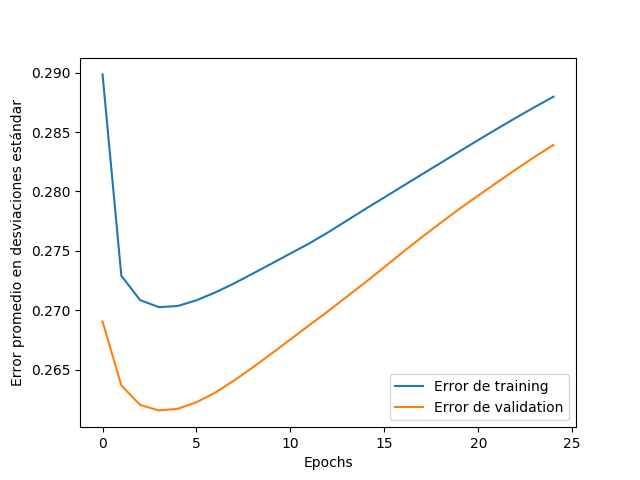
\includegraphics{mlp_imgs/error_eps005.png}
\caption{EPSILON = 0.05}
\end{figure}

\begin{figure}
\centering
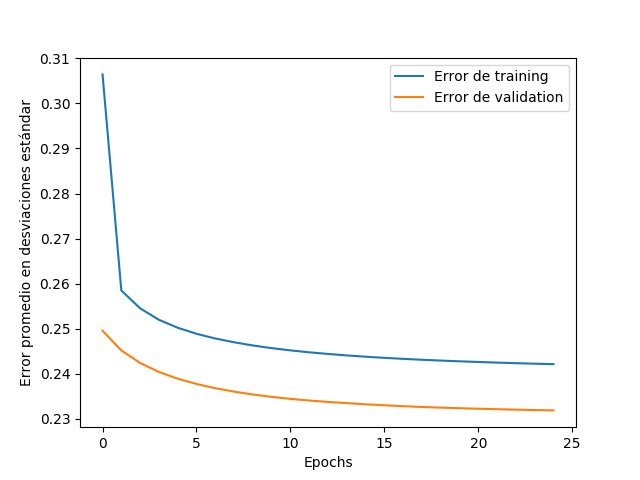
\includegraphics{mlp_imgs/error_eps001.png}
\caption{EPSILON = 0.01}
\end{figure}

Al ver que no era necesario entrenar por tantas epochs dejamos de
entrenar epochs cuando el error relativo entre una epoch y la anterior,
respecto al conjunto de validación fue menor al 1\%. De esta manera se
obtuvo que con 6 epochs fue suficiente.

\begin{figure}
\centering
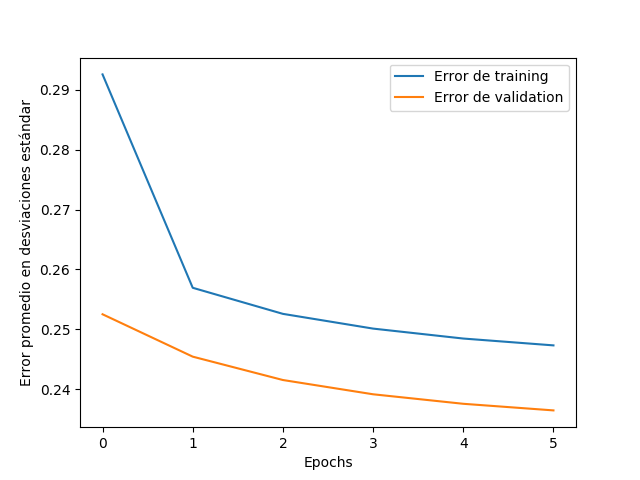
\includegraphics{mlp_imgs/error_eps001_epochsfixed.png}
\caption{EPSILON = 0.01, epochs = 6}
\end{figure}

Sobre el conjunto de test obtuvimos una accuracy de 0.2469, lo que
significa que estuvimos, en promedio, alejados 0.2469 desviaciones
estándar de la media de los valores esperados. En dólares, es un error
absoluto promedio de U\$S 88000, 5\% del precio promedio de las casas.

Para dar un ejemplo, para el último ejemplo del dataset, los precios
son, en desviaciones estándar:

\begin{itemize}
\tightlist
\item
  precio\_real = 0.1894114308541653
\item
  precio\_predicho = 0.23078116332519005
\end{itemize}

Lo que en dólares se traduce a:

\begin{itemize}
\tightlist
\item
  precio\_real = 1298945
\item
  precio\_predicho = 1313556
\end{itemize}

E implica una diferencia de 14611 dólares, lo que es un 1.1\% de
diferencia.

\hypertarget{uso-en-el-control-de-un-puxe9ndulo-invertido}{%
\subsection{Uso en el control de un péndulo
invertido}\label{uso-en-el-control-de-un-puxe9ndulo-invertido}}

En este caso se desea realizar el control de posición del péndulo
invertido trabajado en el TP 2. Allí se realizó un control mediante
lógica difusa en el cual para cada valor de posición y velocidad
angular, se devolvía un valor de fuerza que se debía aplicar. Cada
cierto delta de tiempo se actualizaba el modelo para esa fuerza obtenida
y con los nuevos valores de posición y velocidad se encontraba un nuevo
valor de fuerza. Se proseguía hasta tener el péndulo en posición
vertical, totalmente estable.

Lo que se intenta hacer en este ejercicio es, a partir de un dataset
generado por los valores de posición, velocidad y fuerza obtenidos
mediante el controlador difuso, entrenar la red neuronal y utilizar esta
última como controlador. Así es que al final veremos la performance del
MLP en su intento de estabilizar el péndulo en posición vertical.

\hypertarget{generaciuxf3n-del-dataset}{%
\subsubsection{Generación del dataset}\label{generaciuxf3n-del-dataset}}

Para generar los datos a usar en el entrenamiento, validación y test del
MLP se eligieron 10000 pares de valores ángulo-velocidad de forma
aleatoria con dos distribuciones normales con media cero. Las
desviaciones estándar, para obtener valores dispersos pero
representativos, fueron de pi/3 rad y de 6 rad/s respectivamente. Con
ese par de valores se ingresa al controlador difuso y se guarda el valor
de fuerza en N que devuelve.

El dataset se dividió en entrenamiento (0-6000), validación (6001-8000)
y test (8001-10000) y se le aplicaron los mismos métodos de
normalización que al dataset de USA Housing. De esta forma, todos los
valores están expresados en cantidad de desviaciones estándar por fuera
de la media del campo, ya sea ángulo, velocidad o fuerza (respecto al
conjunto de training).

\hypertarget{entrenamiento}{%
\subsubsection{Entrenamiento}\label{entrenamiento}}

Igual que con el anterior dataset, se variaron el ritmo de aprendizaje y
la cantidad de neuronas en la capa oculta. La variación de este último
parámetro no generó prácticamente ningún impacto en la performance de la
red por lo que se dejó en 15. Se comenzó además con 50 epochs variando
el ritmo de aprendizaje. Encontramos que el mejor valor fue de EPSILON =
0.025 ya que valores menores tardaban mucho en mejorar y valores mayores
comenzaban a diverger. A continuación vemos la gráfica de error vs
epochs para epsilon de 0.075 y 0.025.

\begin{figure}
\centering
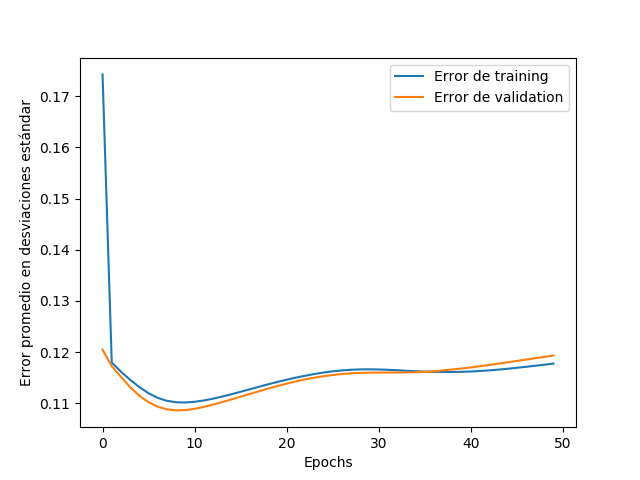
\includegraphics{mlp_imgs/pendulum_50epochs_eps0075.png}
\caption{EPSILON = 0.075}
\end{figure}

\begin{figure}
\centering
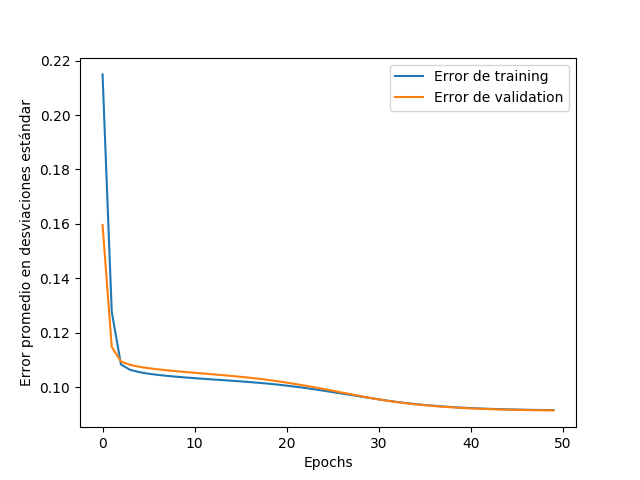
\includegraphics{mlp_imgs/pendulum_50epochs_eps0025.png}
\caption{EPSILON = 0.025}
\end{figure}

Una vez seteado el ritmo de aprendizaje decidimos entrenar epochs hasta
que la diferencia relativa del promedio absoluto del error entre una
epoch y otra, para el conjunto de validación, sea menor al 0.5\%. El
resultado obtenido fue el siguiente

\begin{figure}
\centering
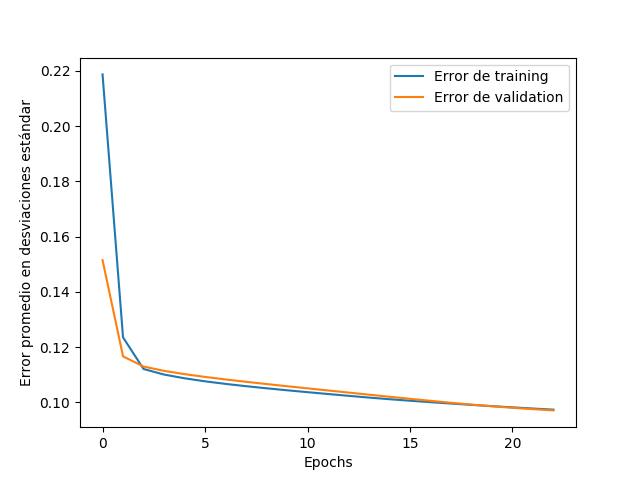
\includegraphics{mlp_imgs/pendulum_epochsfixed_eps0025.png}
\caption{EPSILON = 0.025, epochs = 24}
\end{figure}

El valor de accuracy para el conjunto de test fue de 0.0888, valor
expresado en desviaciones estándar absolutas promedio por encima de la
media. Esto implica un error de 8,88\% desviaciones estándar, lo que
equivale a 3,4N.

\hypertarget{control-del-puxe9ndulo}{%
\subsubsection{Control del péndulo}\label{control-del-puxe9ndulo}}

Finalmente probamos controlar el péndulo con la red neuronal recién
entrenada. Elegimos arbitrariamente una condición inicial de theta =
pi/6 rad = 30° con velocidad inicial nula. En el gráfico vemos posición,
velocidad, y aceleración angulares. Se observa que el control con la red
neuronal no es rápido comparado con el controlador difuso, en el cual en
menos de 2 segundos ya se estabilizaba. Además se puede notar que existe
un pequeño error de estado estable el cual podría ser solucionado
agregandole al controlador una acción integral que lo corrija.

\begin{figure}
\centering
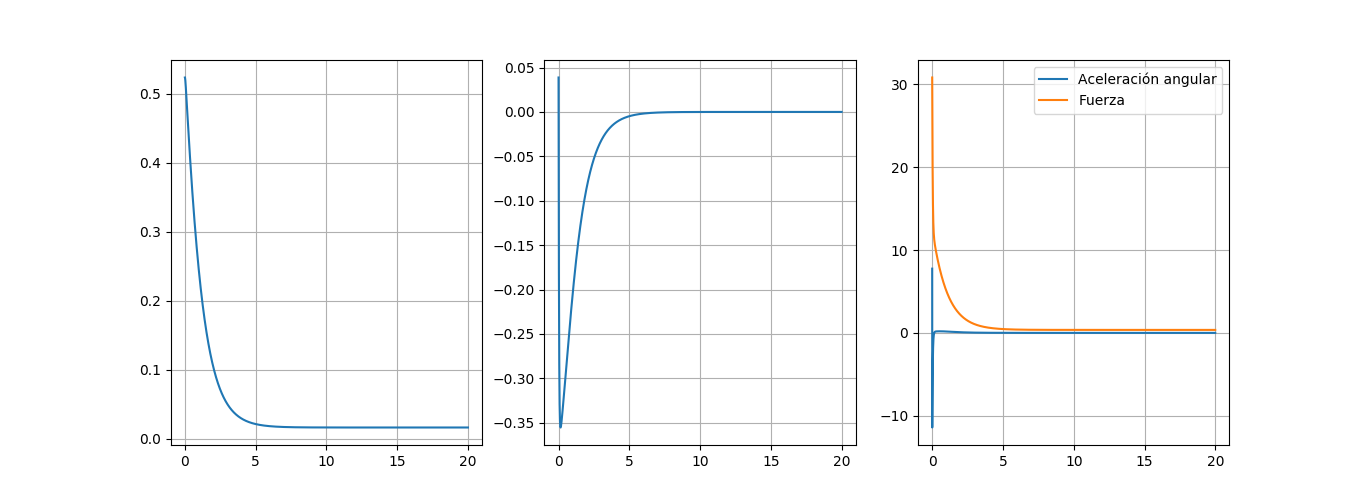
\includegraphics{mlp_imgs/control_pendulo_mlp.png}
\caption{Posición, velocidad y aceleración angulares y fuerza}
\end{figure}

\hypertarget{red-tipo-mapa-de-kohonen}{%
\section{Red tipo mapa de Kohonen}\label{red-tipo-mapa-de-kohonen}}

Implementación de red tipo mapa de Kohonen para reconocer caracteres
manuscritos (clasificación con LVQ) y asociar caracteres parciales con
caracteres completos (memoria asociativa).

\hypertarget{descripciuxf3n-general-de-la-red-neuronal}{%
\subsection{Descripción general de la red
neuronal}\label{descripciuxf3n-general-de-la-red-neuronal}}

\begin{itemize}
\item
  Ritmo de aprendizaje \(\alpha(t)\): Se seleccionó como ritmo de
  aprendizaje una función decreciente linealmente.
\item
  Función de vecindad \(h(|\bar{i}-\bar{g}|, t)\): Se eligió una función
  simple como es la escalón, donde el radio de vecindad R(t) desciende
  linealmente.
\item
  Métrica de similitud: distancia euclídea
\end{itemize}

\hypertarget{acondicionamiento-de-los-datos-de-entrada}{%
\subsection{Acondicionamiento de los datos de
entrada}\label{acondicionamiento-de-los-datos-de-entrada}}

El dataset utilizado es provisto por Keras. Para acondicionar la entrada
del algoritmo, se normalizó los datos entre -1 y 1, dividiendo por 255,
y luego se centró en la media haciendo uso de funciones proveídas por
Numpy.

\hypertarget{divisiuxf3n-del-dataset-en-conjuntos-de-train-y-test}{%
\subsection{División del dataset en conjuntos de train y
test}\label{divisiuxf3n-del-dataset-en-conjuntos-de-train-y-test}}

La primer división del dataset fue en conjunto de entrenamiento y de
testeo. El dataset consta de 60000 imágenes y se destinó aproximadamente
el 30\% a testeo, quedando 39600 imágenes para el entrenamiento de la
red y 20400 para la posterior evaluación final.

Dentro del conjunto de entrenamiento, a su vez se implementó una
evaluación de aprendizaje con \textbf{k-fold cross validation} con k
igual a 3. Esto quiere decir que el conjunto de entrenamiento se dividió
a su vez en subconjunto de entrenamiento y validación, también dejando
el 30\% para validación. Esta división se reliza de 3 formas con los
distintos tercios del conjunto de entrenamiento y se repitió el
experimento 3 veces. Todo esto antes de realizar una última evaluación
de la performance de la red con el conjunto de test.

\hypertarget{arquitectura-de-la-red-neuronal}{%
\subsection{Arquitectura de la red
neuronal}\label{arquitectura-de-la-red-neuronal}}

La red neuronal es una red \textbf{no supervisada} SOFM (Self-Organizing
Feature Maps), con un mapa de 15x15 neuronas (para un mapa de mayor
dimensión el tiempo de ejecución del entranamiento se elevaba demasiado
para los fines prácticos del ejercicio), y donde las entradas serán
vectores de 784 componentes.

La inicialización de los pesos sinápticos se hizo con números aleatorios
entre -1 y 1 utilizando una distribución normal centrada en 0 y sigma
igual a 0,2.

Una vez entrenada la red con el algoritmo básico para SOFM, se realiza
un ajuste fino con LVQ (Learning Vector Quantization) para convertir la
red en una red de clasificación. La inicialización del mapa para LVQ, es
decir el etiquetado de las neuronas del mapa, se realizó dando 10
entradas, una de cada clase, y dando la clase correspondiente a aquellas
neuronas que se activan.

Se intentó realizar esta inicialización con un algoritmo K-means pero no
se obtuvieron mejores resultados.

El mapa entrenado es similar al de la imágen:

\begin{figure}
\centering
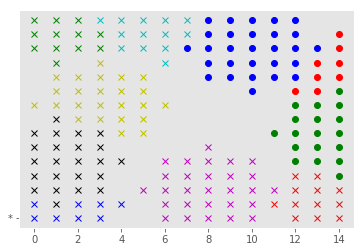
\includegraphics{kohonen_tests/map_kohonen_90-61.png}
\caption{mapa}
\end{figure}

\hypertarget{optimizaciuxf3n-de-hiperparuxe1metros}{%
\subsection{Optimización de
hiperparámetros}\label{optimizaciuxf3n-de-hiperparuxe1metros}}

Para poder elegir los valores de hiperparámetros indicados y subir el
rendimiento de la red, se hizo una optimización muy gruesa dado el
tiempo de ejecución del programa y la cantidad limitada de recursos
computacionales.

\begin{figure}
\centering
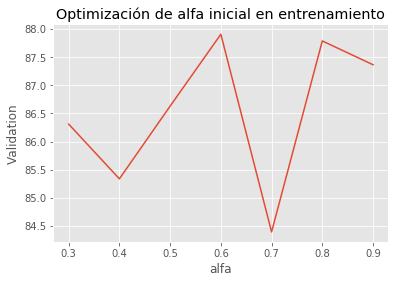
\includegraphics{kohonen_tests/alfa0_train.png}
\caption{alfa0\_train}
\end{figure}

\begin{figure}
\centering
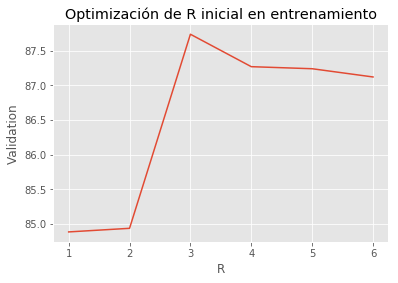
\includegraphics{kohonen_tests/r0_train.png}
\caption{alfa0\_train}
\end{figure}

\begin{figure}
\centering
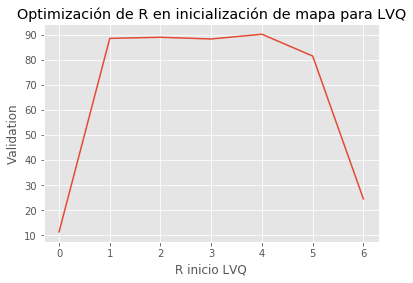
\includegraphics{kohonen_tests/r_init_LVQ.png}
\caption{alfa0\_train}
\end{figure}

\begin{figure}
\centering
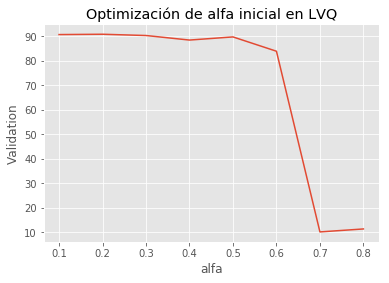
\includegraphics{kohonen_tests/alfa0_lvq.png}
\caption{alfa0\_train}
\end{figure}

\hypertarget{resultados-obtenidos}{%
\subsection{Resultados obtenidos}\label{resultados-obtenidos}}

Los tres experimentos realizados para completar el k-fold, finalizarón
con el siguiente porcentaje de éxito en validación:

\begin{enumerate}
\def\labelenumi{\arabic{enumi})}
\tightlist
\item
  87.47771836007131
\item
  84.97857361493725
\item
  89.13376186103459
\end{enumerate}

Todos porcentajes aceptables para los fines del estudio.

Finalmente una vez entrenado para comparar con el conjunto de test, se
obtuvo el 91.07\% de imágenes clasificados correctamente.

\end{document}
